In this section \textbf{Know}ledge \textbf{D}iscovery \textbf{I}ntegrated \textbf{M}odernization \textbf{E}nvironment (KnowDIME) is presented. The theory behind it is based on the horseshoe modernization model, which is depicts in Figure~\ref{fig:horseshoe}. As can be seen, this model consist of three steps, (\textit{i}) \textbf{Reverse Engineering}, (\textit{ii}) \textbf{Restructuring}, and (\textit{iii}) \textbf{Forward Engineering}. The first step is represented by the left side of the horseshoe, it analyzes the legacy system in order to identify the components of the system and their interrelationships. Usually the reverse engineering step builds one or more representations of the legacy system at a higher level of abstraction (PSM). The second one is represented by the curve of the horseshoe since this steps takes the previous system's representation (PSM) and transforms it into another one (\textbf{P}lataform \textbf{I}ndependent \textbf{M}odel - PIM) at the same abstraction level. Finally, the last step is represented by the right side of the horseshoe because it generates physical implementations (source-code) of the target system at a low abstraction level from the previously restructured representation of the system.

\begin{figure}[!h]
\centering
  % Requires \usepackage{graphicx}%left,bottom, right and top
  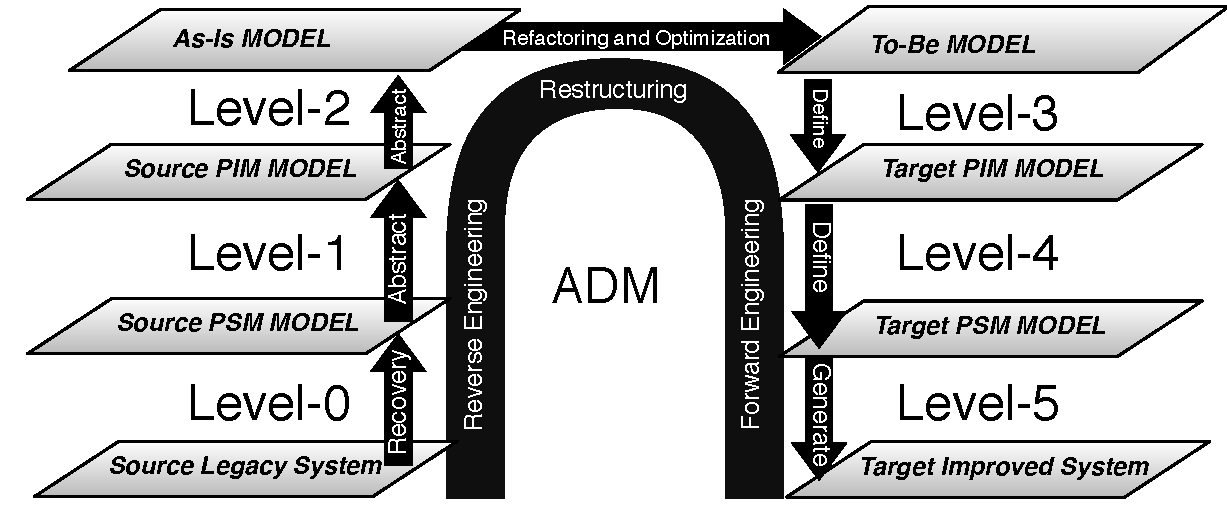
\includegraphics[scale=0.6]{Figuras/horseShoeBOM}
\caption{Horseshoe modernization model.}
\label{fig:horseshoe}
\end{figure}

It worth noticing that KDM is the most essential part of our infrastructure. KDM supplies the representation and management of knowledge extracted by means of reverse engineering from all the different software artifacts of the legacy system. Therefore, the legacy knowledge obtained is then modernized into a target improved system by using the concept of MDD. As the infrastructure herein follows the three steps depicts in Figure~\ref{fig:horseshoe} then it has to go through six abstraction levels with five transformations among them. In Figure~\ref{fig:infra} is depicted the infrastructure and also illustrates all abstract levels and the transformations (see the letters `A'- `F'). The Section~\ref{subsection:abstract_level} describes these abstract levels and the Section~\ref{subsection:transformation} explains the transformations.

\subsection{Abstract Levels}\label{subsection:abstract_level}
The \textbf{Level-0} represents all artifacts of the legacy systems in the real world, such as source code and database. The infrastructure uses this artifacts as input to start the ADM process.

The \textbf{Level-1} consist of two PSM. The former model is a source code model, which represents all abstraction of the legacy system's source code, Figure~\ref{fig:infra}(B) illustrates it. More specifically, this model represents an \textbf{A}bstract \textbf{S}yntax \textbf{T}ree (AST), which is a tree representation of the abstract syntactic structure of Java source code. The latter is a database model that illustrates informations related to database used in the legacy system, see Figure~\ref{fig:infra}(A). Similarly, this model is also represented by an AST, the only difference is that it represents syntactic structure of database instead of Java source code. This database model is based on the SQL-92 Data Manipulation Language which can represent the SQL operations such as \textit{Select}, \textit{Delete}, \textit{Update} and \textit{Insert}. %In order to transform the legacy system in these models it is necessary carry out a syntactical analyzer. As for the first model we used a parser that provides a complete self-describing representation of Java source code, i.e., this representation reflects the structure of the software artifact directly in the nesting of elements. Regarding the second model we devised a SQL parser. It consists of a extension of the previously parser but it intends to identify SQL embedded in the legacy system's source code. This parser focus on identifying SQL operations such as \textit{Select}, \textit{Delete}, \textit{Update} and \textit{Insert}; the tables, the columns, primary keys, etc, that appear in these SQL operations are then represented into a AST. Both models, the source code model and the data base model  are represented in the XMI (\textbf{XM}L Metadata \textbf{I}nterchange)-based syntax as can be seen in Figure~\ref{fig:infra} (B) and Figure~\ref{fig:infra} (A), respectively.   


%Both models are deemed as PSM once they owns the software artifact according to their specific technology platforms. 

The \textbf{Level-2} consist of a combination of the two PSMs (see \textbf{Level-1}) for creating a single `As-Is' PIM which is based on the KDM, Figure~\ref{fig:infra}(C) depicts it. This single model makes possible to represent the artifacts of the legacy systems in an integrated and technological-independent way. %The first PSM (source-code) it is transformed to the KDM Code Package, which represents common program elements supported by various programming languages, such as data types, classes, procedures, and templates. In the same way, the second PSM (database model) it is transformed to the KDM Data Package that represents complex data repositories, such as relational databases. 
Afterwards, in the \textbf{Level-3}, by using this PIM the infrastructure allows the software engineer to realize a set of refactoring, refinement and optimizations in such model in order to meet new requirements. %In other words, a set of automated refactoring operations are carried out against the PIM to generate a redesigned PIM. For instance, the software engineer can pick out if he would like to refactor the legacy system to meet either Data Access Object (DAO) or Service-Oriented Architecture (SOA) or both refactorings. As result, new meta-classes may be added to this PIM model, as well as new meta-attributes and meta-relationship in order to meet these requirements. 

Then in \textbf{Level-4} the infrastructure use the PIM redesigned to generate a target PSM, which is represented by a `To-Be' \textbf{U}nified \textbf{M}odeling \textbf{L}anguage - UML model. This model illustrates the target improved system. Finally, in the \textbf{Level-5} the source-code of the target improved system is generated by using the UML as input.

\subsection{Transformation}\label{subsection:transformation}

The first transformation happens between the \textbf{Level-0} to the \textbf{Level-1}. As previously mentioned, this transformation is carried out by following a set of Text-To-Model (T2M) rules in order to obtains two PSM from legacy system i.e., source code model and database model. To transform the legacy system in these models it is necessary carry out a syntactical analyzer. As for the first model we used a parser that provides a complete self-describing representation of Java source code, i.e., this representation reflects the structure of the software artifact directly in the nesting of elements. Regarding the second model we devised a SQL parser. It consists of a extension of the previously parser but it intends to identify SQL embedded in the legacy system's source code. This parser focus on identifying SQL operations such as \textit{Select}, \textit{Delete}, \textit{Update} and \textit{Insert}; the tables, the columns, primary keys, etc, that appear in these SQL operations are then represented into a AST. Both models, the source code model and the data base model  are represented in the XMI (\textbf{XM}L Metadata \textbf{I}nterchange)-based syntax as can be seen in Figure~\ref{fig:infra} (B) and Figure~\ref{fig:infra} (A), respectively. 

The second transformation is \textbf{Level-1} to \textbf{Level-2}. This transformation is based on a set of Model-To-Model (M2M) patterns to obtain a `As-Is' PIM, which is based on the KDM, see Figure~\ref{fig:infra} (C). This PIM is generated based on the PSMs from \textbf{Level-1}. The first PSM (source-code) is transformed to the KDM Code Package, which represents common program elements supported by various programming languages, such as data types, classes, procedures, and templates. The second PSM (database model) is transformed to the KDM Data Package that represents complex data repositories, such as relational databases.  

The third transformation \textbf{Level-2} to \textbf{Level-3} realizes a set of M2M operations to transform the `As-Is' PIM to a `To-Be' PIM, i.e., model refactorings and model optimizations are realized in the PIM from \textbf{Level-2}. Therefore, a set of automated model refactorings are carried out against the PIM to generate a redesigned PIM. For instance, the software engineer can pick out if he would like to refactor the legacy system to meet either Data Access Object (DAO) or Service-Oriented Architecture (SOA) or both refactorings. As result, new meta-classes may be added to this PIM model, as well as new meta-attributes and meta-relationship in order to meet these requirements. 

The fourth transformation \textbf{Level-3} to \textbf{Level-4} executes a M2M transformation taking as input the PIM and producing as output a model conforming to the KDM models into UML meta model, see Figure~\ref{fig:infra}(D). Finally, the last transformation \textbf{Level-4} to \textbf{Level-5} realizes a set of Model-To-Code (M2C) generation based on design patterns, such as Data Access Object (DAO) or Service-Oriented Architecture (SOA), see Figure~\ref{fig:infra}(E) and Figure~\ref{fig:infra}(F). The generated code can be complemented by the software engineer in accordance with the more detailed specifications of the application business rules, such as the implementation of specific behaviors and features not covered by the code generation.




\begin{figure}[!h]
\centering
  % Requires \usepackage{graphicx}%left,bottom, right and top
 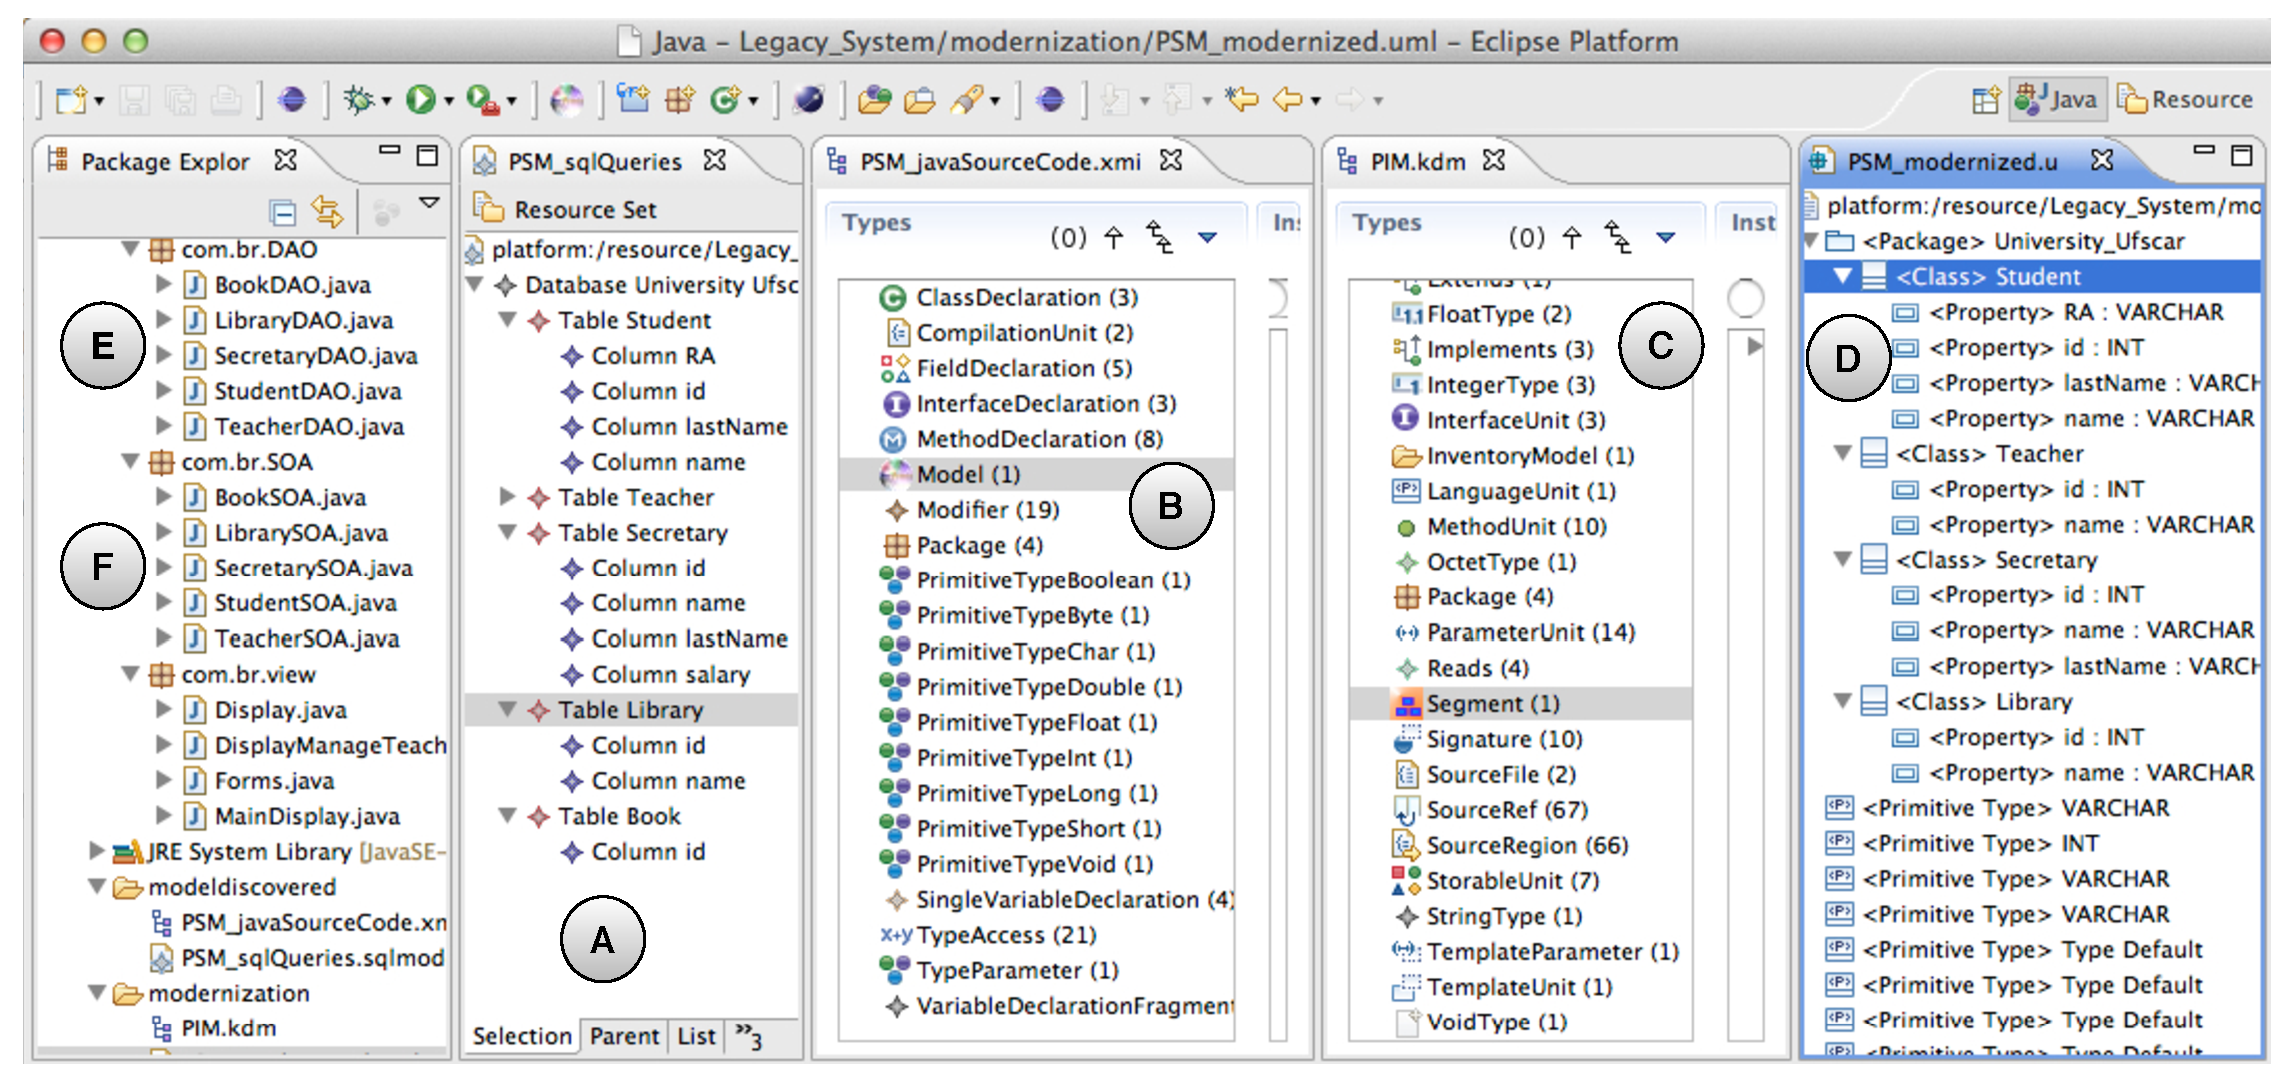
\includegraphics[%scale=0.063, clip=true, trim=32.23cm 18cm 5.45cm 13.853cm
 width=1\textwidth
 ]{Figuras/Tool}
\caption{Screenshot of the KnowDIME}
\label{fig:infra}
\end{figure}